
%(BEGIN_QUESTION)
% Copyright 2013, Tony R. Kuphaldt, released under the Creative Commons Attribution License (v 1.0)
% This means you may do almost anything with this work of mine, so long as you give me proper credit

{\it Shunt resistors} are low-value, precision resistors used as current-measuring elements in high-current circuits.  The idea is to measure the voltage dropped across this precision resistance and use Ohm's Law ($I = {V \over R}$) to infer the amount of current in the circuit:

$$\includegraphics[width=15.5cm]{i03469x01.eps}$$

Since the schematic shows a shunt resistor being used to measure current in an AC circuit, it would be equally appropriate to use an oscilloscope instead of a voltmeter to measure the voltage drop produced by the shunt.  However, we must be careful in connecting the oscilloscope to the shunt because of the inherent ground reference of the oscilloscope's metal case and probe assembly.

Explain why connecting an oscilloscope to the shunt as shown in this second diagram would be a bad idea:

$$\includegraphics[width=15.5cm]{i03469x02.eps}$$

Next, identify a better method of measuring current in this circuit.

\underbar{file i03469}
%(END_QUESTION)





%(BEGIN_ANSWER)

This would be a bad idea because the oscilloscope's ground clip would attempt to bypass current around the shunt resistor, through the oscilloscope's safety ground wire, and back to the grounded terminal of the AC source.  Not only would this induce measurement errors, but it could damage the oscilloscope as well.

The ground-referenced clip on an oscilloscope probe is a constant source of potential trouble for those who do not fully understand it!  Even in scenarios where there is little or no potential for equipment damage, placing an earth ground reference on a circuit via the probe clip can make for very strange circuit behavior and erroneous measurements.  Problems like this frequently occur when new students attempt to connect their oscilloscopes to circuits powered by signal generators whose outputs are also earth-ground referenced.

\vskip 10pt

As for a better test technique, the most obvious answer is to reverse the probe connections: ground clip on the left-hand terminal and probe tip on the right-hand terminal.  However, even this might not be the best idea, since it creates a ``ground loop'' between the oscilloscope and the ground connection at the AC source:

$$\includegraphics[width=15.5cm]{i03469x03.eps}$$

\filbreak

Ground loops are to be avoided in measurement circuits because they may be the source of some very strange effects, including the coupling of noise voltage from entirely unrelated circuits to the one being measured.  To avoid this problem, the best solution for measuring the voltage dropped across the shunt resistor is to use two scope probes and set the scope up for {\it differential} voltage measurement:

$$\includegraphics[width=15.5cm]{i03469x04.eps}$$

%(END_ANSWER)





%(BEGIN_NOTES)


%INDEX% Electronics review: oscilloscope usage

%(END_NOTES)


